% WACV 2027 Paper Template
% based on the ICCV 2025 template (https://media.eventhosts.cc/Conferences/ICCV2025/ICCV2025-Author-Kit-Feb.zip) with
% WACV-specific details (e.g., 2 tracks) from the WACV 2025 template (https://www.dropbox.com/scl/fi/su44zgdhrzik26p2xu37k/WACV-2025-Author-Kit-Template.zip?rlkey=5qcfimjhxnmx3wlyk7yhk8wg7&dl=0)

\documentclass[10pt,twocolumn,letterpaper]{article}

%%%%%%%%% PAPER TYPE  - PLEASE UPDATE FOR FINAL VERSION
\usepackage[review,algorithms]{wacv}      % To produce the REVIEW version for the algorithms track
% \usepackage[review,applications]{wacv}      % To produce the REVIEW version for the applications track
% \usepackage[review,datasets]{wacv}      % To produce the REVIEW version for the datasets track
% \usepackage{wacv}              % To produce the CAMERA-READY version
%\usepackage[pagenumbers]{wacv} % To force page numbers, e.g. for an arXiv version

% Import additional packages in the preamble file, before hyperref
%
% --- inline annotations
%
\newcommand{\red}[1]{{\color{red}#1}}
\newcommand{\todo}[1]{{\color{red}#1}}
\newcommand{\TODO}[1]{\textbf{\color{red}[TODO: #1]}}
% --- disable by uncommenting  
% \renewcommand{\TODO}[1]{}
% \renewcommand{\todo}[1]{#1}


\usepackage{booktabs}


% It is strongly recommended to use hyperref, especially for the review version.
% hyperref with option pagebackref eases the reviewers' job.
% Please disable hyperref *only* if you encounter grave issues, 
% e.g. with the file validation for the camera-ready version.
%
% If you comment hyperref and then uncomment it, you should delete *.aux before re-running LaTeX.
% (Or just hit 'q' on the first LaTeX run, let it finish, and you should be clear).
\definecolor{wacvblue}{rgb}{0.21,0.49,0.74}
\usepackage[pagebackref,breaklinks,colorlinks,allcolors=wacvblue]{hyperref}

%%%%%%%%% PAPER ID  - PLEASE UPDATE
\def\wacvPaperID{*****} % *** Enter the WACV Paper ID here
\def\confName{WACV}
\def\confYear{2027}


%%%%%%%%% TITLE - PLEASE UPDATE
\title{Would Imagination Help? An Oracle Study of Visual Intermediate States\\for Spatial and Physical Reasoning in VLMs}

%%%%%%%%% AUTHORS - PLEASE UPDATE
\author{Anonymous WACV LVR Workshop Submission}

\begin{document}
% teaser directly under the title block, as in CVPR-style papers
\twocolumn[{\renewcommand\twocolumn[1][]{#1}\maketitle
\begin{center}
  \vspace{-1.5em}
  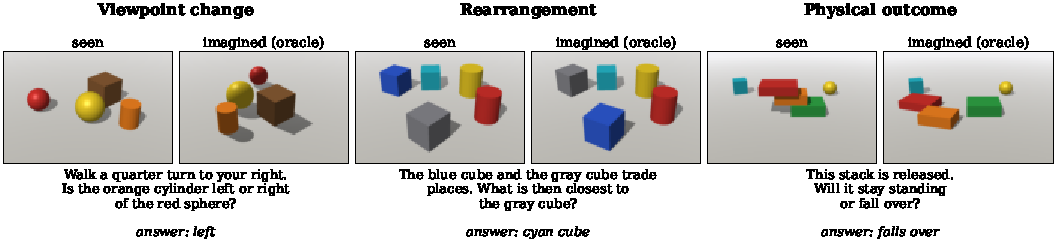
\includegraphics[width=\linewidth]{figs/teaser.pdf}
  \captionof{figure}{\textbf{Each question asks the model to picture a change it cannot see.} Because our scenes are rendered from an exact 3D description, we can render the state the question asks about (``imagined (oracle)''), a plausible but misleading version of it, or the model's own reconstruction, and give any of them back to the model as a second image.}
  \label{fig:teaser}
  \vspace{1em}
\end{center}}]
\begin{abstract}
Vision-language models usually reason about change in text. Would they do better if they could \emph{see} the changed scene? We build a benchmark in which the state a question asks about (the view from another position, the scene after two objects trade places, or the outcome of releasing a stack of blocks) can be rendered exactly, and give it to the model as a second image. Across three open VLMs from two families, a perfect imagined state raises accuracy on every task, by up to 30 points, while describing the change in text first gives a significant gain in only one case, a question that can be restated in terms of the visible scene. On viewpoint questions, a misleading imagined state drops accuracy far below the image-only baseline, and models then give the answer it implies up to 81\% of the time, so the visual state plays a causal role. Imagination need not be precise: an oracle with 1\,m of position noise still helps on viewpoint questions. Yet models gain little from their own imagined states, partly because they misperceive the relations that matter and partly because they do not rely on what they produced. Finally, the seen image competes with the imagined one: on viewpoint questions whose answer changes after moving, models answer 90--98\% correctly from the imagined view alone but only 29--61\% when the original image is also shown.
\end{abstract}

\section{Introduction}
\label{sec:intro}

Asked what happens if you walk around a table, or whether a leaning stack of blocks will hold, people tend to picture the result rather than reason it out in words. Vision-language models (VLMs) usually do the opposite: they encode the image once and carry out every intermediate step in text. Several recent methods give models a visual intermediate state instead, by drawing sketches~\cite{hu2024sketchpad}, by producing latent visual tokens~\cite{yang2026mirage,li2025lvr}, or by supplying extra views~\cite{wang2026mindcube}. These methods change many things at once (training data, architecture, compute), so it is hard to tell whether the visual state itself is what helps.

We isolate that one factor. We build scenes in which the imagined state a question asks about can be \emph{rendered exactly} (\cref{fig:teaser}): the view from where the viewer would stand, the scene after two objects trade places, or the aftermath of releasing a stack of blocks. We then hold the model, the question and the prompt fixed and vary only the second image the model receives. This lets us ask three questions:
\begin{enumerate}[nosep,leftmargin=*]
  \item \textbf{How much would perfect imagination help?} An exact rendering of the imagined state (the oracle) is a reference point for methods that produce a visual intermediate state, under our rendering and prompt protocol.
  \item \textbf{Does the model actually use it?} Replacing the oracle with a misleading or an unrelated image tests whether the answer depends on what the visual state shows, rather than on having a second image at all.
  \item \textbf{How faithful must imagination be, and how close do models get on their own?} We degrade the oracle with controlled position noise, and we let the model build its own imagined state by writing down the scene and rendering it.
\end{enumerate}

Across four open VLMs, the answers to these questions differ by task, and in the 7--8B models the seen image competes with the imagined one (\cref{sec:results}). Code, data and the supplementary material (prompts, further controls, all significance tests) are at \url{https://github.com/Lkumar209/lvr-imagination}.

\section{Related Work}
\label{sec:related}

\paragraph{Visual intermediate states.} Visual Sketchpad~\cite{hu2024sketchpad} lets a model draw on the image with tools and look again. Mirage~\cite{yang2026mirage} and Latent Visual Reasoning~\cite{li2025lvr} train models to emit latent visual tokens between text steps. MindCube~\cite{wang2026mindcube} finds that supplying unseen intermediate views, or having the model write a cognitive map first, improves spatial reasoning from limited views. Our study is complementary: instead of proposing a method, we measure the ceiling that any such method could reach on our tasks, test with interventions whether the intermediate image is causally used, and quantify how much error it can tolerate.

\paragraph{Spatial and physical reasoning in VLMs.} VLMs struggle with basic spatial relations~\cite{kamath2023whatsup} and with perceptual tasks humans solve at a glance~\cite{fu2024blink}. Recent work reports a strong egocentric bias in perspective taking, with most errors reproducing the camera's own view~\cite{wang2026egocentric}; we observe the same bias and show that an imagined view removes much of it. Our scenes follow the synthetic, fully controlled style of CLEVR~\cite{johnson2017clevr}, and our stability task follows the block-tower setting of Lerer \etal~\cite{lerer2016blocks}.

\section{Benchmark and Protocol}
\label{sec:benchmark}

\begin{figure*}[t]
  \centering
  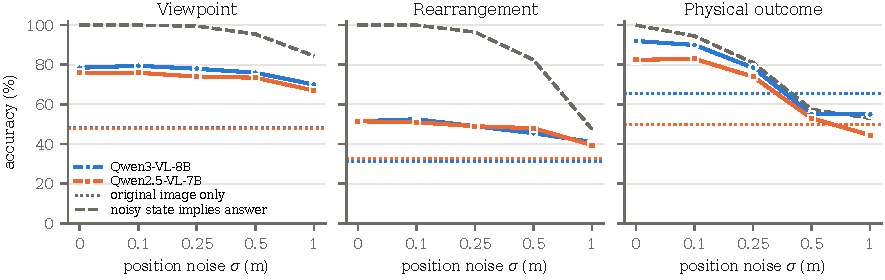
\includegraphics[width=\linewidth]{figs/noise.pdf}
  \caption{\textbf{Accuracy with a degraded oracle} (Qwen models). Solid: accuracy when the imagined state is rendered from object positions perturbed with Gaussian noise $\sigma$. Dotted: the same model with the original image only. Gray dashed: how often the perturbed state still implies the correct answer.}
  \label{fig:noise}
\end{figure*}

\paragraph{Scenes and rendering.} Scenes contain 4--6 spheres, cubes and cylinders on a floor, each with a unique color, rendered at $448{\times}448$ pixels with a 40$^\circ$ field of view by a small ray tracer with shadows. Every scene is an exact 3D description, so any changed state can be rendered without approximation.

\paragraph{Tasks.} We generate 200 questions for each of three tasks (\cref{fig:teaser}). \emph{Viewpoint}: after walking a quarter or half way around the scene, is object A to the left or right of object B? \emph{Rearrangement}: after A trades places with B, which object is closest to A? \emph{Physical outcome}: will a stack of 3--4 offset blocks stay standing when released? Stability follows from the center of mass of each sub-stack relative to its support. Answers are computed from geometry, with margins that exclude borderline cases (a screen-space gap of at least 8\% of the image width; a nearest/second-nearest distance ratio of at least 1.4; a center of mass at least 8\,cm from any tipping edge).

\paragraph{Shortcut controls.} Binary answers are balanced by construction. For viewpoint, half the questions have an answer that differs from the one in the current view, so answering from the current view scores 50\%. For rearrangement, the answer is never the swap partner nor the target's nearest neighbor before the swap.

\paragraph{Conditions.} The model always sees the original image and the question, and answers with one option. \textbf{Img.}: nothing else. \textbf{Text}: it first describes the changed scene in words. \textbf{Oracle}: a second image shows the exact imagined state. \textbf{Misl.}: the second image shows a plausible imagined state with a different answer (another viewpoint, another swap, the opposite outcome). \textbf{Unrel.}: the second image is the oracle of a different question of the same task. \textbf{Oracle alone}: the imagined state replaces the original image, with its own wording (supplementary). \textbf{Own}: the model first lists every object and its floor position as JSON; we apply the change described in the question and render the result as the second image. All two-image conditions use identical wording, so the model cannot tell them apart from the prompt.

\paragraph{Models.} Qwen3-VL-8B-Instruct~\cite{qwen2025qwen3vl}, Qwen2.5-VL-7B-Instruct~\cite{bai2025qwen25vl} and InternVL3-8B~\cite{zhu2025internvl3}, all with 4-bit NF4 weights, Qwen3-VL-32B-Instruct (4-bit, without Text and Own), and Qwen2.5-VL-3B-Instruct in bf16 as a smaller reference; greedy decoding. Because of its length, ``Text'' is run on 100 questions per task (Qwen2.5-VL-7B: all 200; Qwen3-VL-8B: 200 on rearrangement). We report accuracy, and compare conditions on the same questions with exact McNemar tests, Holm-corrected over all comparisons.

\section{Results}
\label{sec:results}

\begin{table}[t]
  \centering
  \small
  \setlength{\tabcolsep}{3.2pt}
  \resizebox{\linewidth}{!}{\begin{tabular}{lcccccc}
\toprule
 & \multicolumn{3}{c}{Qwen3-VL-8B} & \multicolumn{3}{c}{Qwen2.5-VL-7B} \\
\cmidrule(lr){2-4}\cmidrule(lr){5-7}
Second input & View & Swap & Stab. & View & Swap & Stab. \\
\midrule
Original image only & 48.5 & 31.0 & 65.5 & 48.0 & 32.5 & 50.0 \\
+ describe the change in text$^\dagger$ & 61.0 & \textbf{64.0} & 52.0 & 56.0 & 38.0 & 46.5 \\
+ own imagined state & 52.0 & 36.0 & 55.0 & 52.5 & 37.0 & 46.5 \\
+ oracle imagined state & \textbf{78.5} & 51.5 & \textbf{93.0} & \textbf{76.0} & \textbf{51.5} & \textbf{80.0} \\
+ another question's state & 50.0 & 34.5 & 54.0 & 49.5 & 28.0 & 49.5 \\
\midrule
+ misleading imagined state & 19.5 & 35.5 & 19.5 & 24.5 & 34.5 & 42.5 \\
\quad \emph{answers as the misleading state implies} & 80.5 & 28.0 & 80.5 & 75.5 & 36.5 & 57.5 \\
\bottomrule
\end{tabular}
}
  \caption{\textbf{Accuracy (\%) by second input}, 200 questions per task (chance: 50 / 29 / 50). Img.: original image only. Text: describe the change in words first. Own: the model's own imagined state. Oracle: the exact imagined state. Unrel.: another question's imagined state. Misl.: a misleading imagined state. Follows: how often the model gives the answer the misleading state implies. Best per row in bold (excluding Misl.). $^\dagger$Fewer questions (100--200 per task) for Text.}
  \label{tab:main}
\end{table}

\paragraph{Perfect imagination helps.} The oracle imagined state raises accuracy on every task for all three models (\cref{tab:main}): by 20--30 points for the two Qwen models and by 8--11 points for InternVL3-8B. All nine gains are significant (exact McNemar test, Holm-corrected over all comparisons, $p<0.05$; supplementary). An unrelated imagined state stays within 5 points of the image-only baseline, or lowers it (Qwen3-VL-8B, physical outcome: 65.5\,$\rightarrow$\,54.0), so the gain comes from the content of the image, not from a second image as such. The benefit also needs a model that can read the imagined state: the smaller Qwen2.5-VL-3B is near chance even on the imagined view alone (viewpoint: 52.5\%), and gains little from the oracle (47.5\,$\rightarrow$\,55.5). The pattern is unchanged under a paraphrased prompt with the options reversed (supplementary).

\paragraph{The model uses the imagined state.} A misleading imagined state lowers viewpoint accuracy below the image-only baseline for all three models (Qwen3-VL-8B 48.5\,$\rightarrow$\,19.5, Qwen2.5-VL-7B 48.0\,$\rightarrow$\,24.5, InternVL3-8B 51.0\,$\rightarrow$\,37.0, all significant), and the models then give the answer the misleading state implies 63--81\% of the time. Qwen3-VL-8B shows the same on physical outcome (65.5\,$\rightarrow$\,19.5; follows 80.5\%). The visual intermediate state therefore plays a causal role. The effect is weaker or absent where the image is harder to read (rearrangement) or where the model mostly ignores it (InternVL3-8B on physical outcome, which answers ``falls over'' for nearly every stack whenever a second image is given).

\paragraph{The seen image competes with the imagined one.} With the original image only, all three models answer viewpoint questions from their current view: accuracy is 78--99\% when the answer does not change after moving but 3--19\% when it does, matching the egocentric bias reported by Wang \etal~\cite{wang2026egocentric}. Given the imagined view \emph{alone}, they solve these hard cases (90--98\%). Given both images, they fall back to 61\% (Qwen3-VL-8B), 53\% (Qwen2.5-VL-7B) and 29\% (InternVL3-8B): the original image pulls the answer back towards the current view, by a different amount for each model. A method that produces a visual intermediate state must therefore also get the model to rely on it.

\paragraph{When does text reasoning suffice?} Describing the change in words first (``Text''; for Qwen3-VL-8B a mean of 646 generated tokens per answer, median 461, against at most 5 otherwise) gives a significant gain in one case only: Qwen3-VL-8B on rearrangement (31.0\,$\rightarrow$\,61.5), where it matches the oracle (51.5; difference not significant). Its reasoning rewrites ``closest to A after A and B trade places'' as ``closest to B's current position, apart from A'', which can be read from the original image without imagining anything. For viewpoint and physical outcome, no model gains significantly from text, while the oracle helps every model. Text suffices when a question can be re-expressed in terms of the visible scene; otherwise the imagined state is what helps.

\paragraph{How faithful must imagination be?} \Cref{fig:noise} adds Gaussian noise to every object's position before rendering the oracle (Qwen models). Viewpoint and rearrangement are forgiving: with $\sigma{=}1$\,m, Qwen3-VL-8B still reaches 70.0 and 41.0, above its image-only 48.5 and 31.0 (Qwen2.5-VL-7B: 67.0 and 39.5 vs.\ 48.0 and 32.5). Physical outcome is fragile, and accuracy follows how often the noisy state still implies the right outcome, falling to chance by $\sigma{=}0.5$\,m.

\begin{figure}[t]
  \centering
  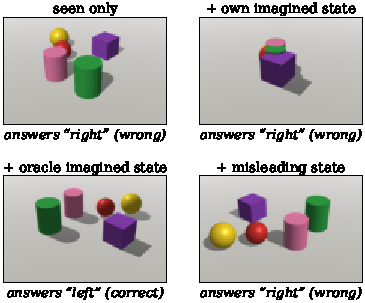
\includegraphics[width=\linewidth]{figs/qual.pdf}
  \caption{\textbf{One question, four second images} (Qwen3-VL-8B, actual answers). ``Walk a quarter turn to your right: is the green cylinder left or right of the red sphere?'' (answer: left). The model's own imagined state piles the objects together, so it does not help; the oracle does, and the misleading state flips the answer back.}
  \label{fig:qual}
\end{figure}

\paragraph{The model's own imagination is limited by perception.} When the model writes the scene down and we render the change, accuracy does not change significantly from the image-only baseline for any model or task (\cref{tab:main}, ``Own''; \cref{fig:qual}). Its reconstruction is worse than an oracle perturbed by 1\,m of noise (Qwen3-VL-8B, viewpoint: 52.0 vs.\ 70.0), because its errors are not random: it implies the correct viewpoint answer only 65\% of the time, and rescaling its layout to the true scene size does not change that (66\%). The failure is perception, not reasoning. On physical outcome, Qwen3-VL-8B answers correctly 96\% of the time when its own reconstruction implies the right outcome and 7.5\% when it does not, following its imagined state 94.5\% of the time, but its reconstruction is right only 53.5\% of the time.

\section{Discussion and Limitations}
\label{sec:discussion}

Our results separate three requirements for reasoning through a visual intermediate state: the state must be \emph{correct in its relations}, though not necessarily precise; the model must \emph{read} it, which it does well on viewpoint and stability and less well on rearrangement; and the model must \emph{rely} on it rather than on the original image. Current VLMs meet the second requirement, but not the first or the third. Text reasoning is not always worse: when a question can be rephrased in terms of what is already visible, it does as well or better, at a much higher token cost. A system that routes between the two would need to recognise which case it is in. Beyond routing, two directions follow: training signals for relational accuracy of the imagined state, and mechanisms that let the imagined state override the observation it was derived from.

\paragraph{Limitations.} Our scenes are synthetic and simple, which is what makes the oracle exact; real scenes would add perception difficulty on top. The physical aftermath is a plausible depiction, not a simulation, and for stable stacks the imagined image equals the original. Given only the aftermath, models answer with a fixed prior, so we do not interpret imagined-only accuracy on that task. We evaluate two open 7--8B models with 4-bit weights; larger models may rely on the imagined state differently.

{
    \small
    \bibliographystyle{ieeenat_fullname}
    \bibliography{main}
}

% supplementary material: after the references, does not count towards the page limit
\clearpage
\onecolumn
\appendix
\section{Prompts}
\label{sec:supp-prompts}
All prompts are shown for the viewpoint question of \cref{fig:teaser}; the other tasks differ only in the task-specific sentence, listed after. Images are passed before the text.

\paragraph{direct} (one image: the original)
\begingroup\footnotesize\begin{verbatim}
The image shows a scene.

Imagine you walk a quarter of the way around the scene to your right, keeping
your eyes on the center of the scene. From that new viewpoint, is the orange
cylinder to the left or to the right of the red sphere?
Options: left / right

Reply with only a single line of the form 'Answer: <option>'.
\end{verbatim}
\endgroup
\paragraph{oracle, wrong, shuffled, recon} (two images: the original, then the imagined state). The wording is identical across these four conditions.
\begingroup\footnotesize\begin{verbatim}
The first image shows the current scene. The second image shows the scene from
the new viewpoint described in the question.

Imagine you walk a quarter of the way around the scene to your right, keeping
your eyes on the center of the scene. From that new viewpoint, is the orange
cylinder to the left or to the right of the red sphere?
Options: left / right

Reply with only a single line of the form 'Answer: <option>'.
\end{verbatim}
\endgroup
\paragraph{oracle alone} (one image: the imagined state) The first line of \emph{direct} becomes:
\begingroup\footnotesize\begin{verbatim}
The image shows the scene from the new viewpoint described in the question.
\end{verbatim}
\endgroup
\noindent and analogously for the other tasks (``The image shows the scene after\ldots'').

\paragraph{cot} The last line of \emph{direct} is replaced by a task-specific instruction followed by \texttt{End your reply with a final line of the form 'Answer: <option>'.} The instructions are:
\begingroup\footnotesize\begin{verbatim}
viewpoint: First describe, step by step, how the scene would look from the new
viewpoint, then answer.
swap: First describe, step by step, where every object would be after the
swap, then answer.
stability: First reason, step by step, about where the weight of the upper
blocks rests and what would happen after release, then answer.
\end{verbatim}
\endgroup
\paragraph{Second-image sentence for the other tasks.}
\begingroup\footnotesize
\begin{verbatim}
swap:      The second image shows the scene after the two objects have
           traded places.
stability: The second image shows the scene after the stack was released
           and everything came to rest.
\end{verbatim}
\endgroup
\paragraph{Reconstruction (recon, first stage).} Viewpoint and rearrangement:
\begingroup\footnotesize\begin{verbatim}
List every object in the image. For each one give its name as '<color>
<shape>' (shape is one of: cube, sphere, cylinder) and where it stands on the
floor, seen from above, in meters: x runs from left (negative) to right
(positive) as seen in the image, and z runs from far away (negative) to close
to the camera (positive). All objects are within about 2.5 m of the center of
the scene. Reply with only a JSON list, for example [{"name": "red cube", "x":
0.5, "z": -1.0}, {"name": "blue sphere", "x": -1.2, "z": 0.8}]
\end{verbatim}
\endgroup
Physical outcome:
\begingroup\footnotesize\begin{verbatim}
Look at the stack of flat blocks (ignore any objects lying apart from the
stack). List the blocks from the bottom of the stack to the top. For each give
its color, its width in meters (blocks are 0.9 to 1.5 m wide), and the
horizontal position of its center in meters, from left (negative) to right
(positive) as seen in the image. Reply with only a JSON list, for example
[{"color": "red", "width": 1.2, "x": 0.0}, {"color": "blue", "width": 1.0,
"x": 0.3}]
\end{verbatim}
\endgroup
When a reconstruction leaves out one of the two swapped objects, no imagined state can be rendered and the question is answered from the original image only. This happens on rearrangement for 18 (Qwen3-VL-8B), 3 (Qwen2.5-VL-7B) and 11 (InternVL3-8B) of 200 questions, and never on the other tasks.

Answers are parsed from the last \texttt{Answer:} line, falling back to the last option mentioned anywhere in the reply. Decoding is greedy; the answer limit is 48 new tokens. For \emph{cot} it is 1{,}024; answers that reached it were regenerated with 2{,}048, which under greedy decoding is equivalent to a 2{,}048 limit throughout. For Qwen3-VL-8B, 35 of the first 300 \emph{cot} answers reached 1{,}024 tokens; regenerating them left the number of correct answers unchanged (11), and 14 of them reached 2{,}048 as well, mostly by repeating themselves.

\paragraph{Use of language models.} Besides the VLMs under study, an LLM-based coding assistant was used to help implement the scene generator, renderer and evaluation code, to run and monitor experiments, and to draft and edit text. The authors checked the code, the results and every number and citation in the paper.

\section{Dataset details}
\label{sec:supp-data}
\begin{table}[h]
\centering\small
\begin{tabular}{lccc}
\toprule
 & Viewpoint & Rearrangement & Physical outcome \\
\midrule
Questions & 200 & 200 & 200 \\
Objects per scene & 4--6 (mean 5.0) & 5--6 (mean 5.5) & 3--4 blocks + 1--2 others \\
Options & 2 & 3--4 & 2 \\
Answer balance & 100 left / 100 right & -- & 100 stand / 100 fall \\
Other & \multicolumn{3}{l}{\footnotesize moves: 91 right, 75 left, 34 opposite; 100 flip the current-view answer} \\
\bottomrule
\end{tabular}
\end{table}
\noindent Rearrangement: nearest/second-nearest distance ratio at least 1.4 (median 1.6). Physical outcome: 133 three-block and 67 four-block stacks; unstable stacks fail at the base (69) or at the second block (31). The misleading state is another viewpoint with the opposite answer (viewpoint), a swap with a different partner and a different answer (rearrangement), or the opposite outcome (physical outcome; for stable stacks, the top block falls toward its overhang). Rearrangement answers are skewed toward cylinders (41\% of answers but 33\% of options), so a guesser that prefers cylinders would score about 35\% rather than 29\%.

\section{Additional results}
\label{sec:supp-results}

\paragraph{Egocentric bias by model.} Viewpoint accuracy (\%) on questions whose answer is the \emph{same} from the current view and from the new one, and on those where it \emph{flips}. All models answer from the current view when given only the original image; the imagined view alone resolves this for the 7--8B models, and adding the original image back brings much of the bias back.
\begin{center}\small\begin{tabular}{lcccccc}
\toprule
 & \multicolumn{2}{c}{Img.} & \multicolumn{2}{c}{Img.\ + oracle} & \multicolumn{2}{c}{Oracle only} \\
\cmidrule(lr){2-3}\cmidrule(lr){4-5}\cmidrule(lr){6-7}
Model & same & flip & same & flip & same & flip \\
\midrule
Qwen3-VL-8B & 78.0 & 19.0 & 96.0 & 61.0 & 96.0 & 90.0 \\
Qwen2.5-VL-7B & 93.0 & 3.0 & 99.0 & 53.0 & 97.0 & 98.0 \\
InternVL3-8B & 99.0 & 3.0 & 95.0 & 29.0 & 98.0 & 97.0 \\
Qwen2.5-VL-3B & 54.0 & 41.0 & 60.0 & 51.0 & 50.0 & 55.0 \\
\bottomrule
\end{tabular}
\end{center}

\paragraph{Prompt robustness.} Qwen3-VL-8B on the first 50 questions per task, with the original prompt and with a paraphrase that rewords every instruction and lists the options in reverse order. Individual answers change, most on rearrangement. Under both wordings the oracle helps on all three tasks, and the misleading state hurts on viewpoint and physical outcome but not on rearrangement. The image-only baseline on physical outcome also moves (68 to 52), so at $n=50$ these are coarse checks.
\begin{center}\small\begin{tabular}{lcccccc}
\toprule
 & \multicolumn{2}{c}{View} & \multicolumn{2}{c}{Swap} & \multicolumn{2}{c}{Stab.} \\
\cmidrule(lr){2-3}\cmidrule(lr){4-5}\cmidrule(lr){6-7}
Second input & orig. & para. & orig. & para. & orig. & para. \\
\midrule
Img. & 52.0 & 58.0 & 24.0 & 20.0 & 68.0 & 52.0 \\
Oracle & 66.0 & 70.0 & 42.0 & 50.0 & 96.0 & 88.0 \\
Misl. & 22.0 & 28.0 & 32.0 & 32.0 & 20.0 & 38.0 \\
\bottomrule
\end{tabular}
\end{center}

\paragraph{Stability controls.} In the main runs, the oracle for stable stacks and the misleading image for falling stacks are copies of the original. We therefore re-render both second images from a camera turned by 20$^\circ$ around the stack (same scenes, same prompt), so that no second image equals the original. Accuracy (\%) on stable (``stands'') and falling (``falls'') stacks, 100 each:
\begin{center}\small\begin{tabular}{llcccccc}
\toprule
 & & \multicolumn{3}{c}{Oracle} & \multicolumn{3}{c}{Misl.} \\
\cmidrule(lr){3-5}\cmidrule(lr){6-8}
Model & Camera & stands & falls & all & stands & falls & all \\
\midrule
Qwen3-VL-8B & same & 100.0 & 86.0 & 93.0 & 39.0 & 0.0 & 19.5 \\
 & turned & 90.0 & 81.0 & 85.5 & 28.0 & 22.0 & 25.0 \\
Qwen2.5-VL-7B & same & 100.0 & 60.0 & 80.0 & 85.0 & 0.0 & 42.5 \\
 & turned & 100.0 & 48.0 & 74.0 & 55.0 & 0.0 & 27.5 \\
InternVL3-8B & same & 17.0 & 100.0 & 58.5 & 0.0 & 100.0 & 50.0 \\
 & turned & 5.0 & 100.0 & 52.5 & 0.0 & 100.0 & 50.0 \\
\bottomrule
\end{tabular}
\end{center}
A model that only checked whether the picture changed would answer ``falls over'' for every turned image; the Qwen models do not. As a second check, Qwen3-VL-8B's own reconstructions that show a standing stack (189 of 200) differ from the original in about 6\% of the pixels (range 2.0--11.9\%; a pixel counts as changed when a channel differs by more than 30/255), against about 9\% for the fallen-block oracles (range 6.5--12.3\%). Qwen3-VL-8B says ``stays standing'' for 97.4\% of these reconstructions, and for 94.9\% of the 59 that change as much as some fallen-block oracle; in that shared range, the fallen-block oracles get ``falls over'' 85.9\% of the time. The same amount of change thus leads to opposite answers, depending on what the image shows.

\paragraph{Text traces.} The rearrangement count in \cref{sec:results} is a keyword match on Qwen3-VL-8B's replies: a trace counts when it refers to the swap partner's original position (\eg ``where the green sphere was'', ``the original position of the green sphere''); 198 of 200 do.

\medskip\noindent\begin{minipage}{\linewidth}
\paragraph{A smaller model.} Qwen2.5-VL-3B (bf16) stays near chance in every condition, including the imagined state alone, so it cannot benefit from imagination.
\begin{center}\small\begin{tabular}{lcccccc}
\toprule
Task & Img. & Own & Oracle & Oracle only & Unrel. & Misl. \\
\midrule
View & 47.5 & 49.0 & 55.5 & 52.5 & 51.0 & 43.0 \\
Swap & 32.0 & 33.0 & 39.0 & 42.0 & 36.5 & 36.5 \\
Stab. & 50.0 & 49.0 & 51.0 & 49.5 & 50.0 & 50.0 \\
\bottomrule
\end{tabular}
\end{center}
\end{minipage}

\paragraph{Rescaled reconstructions.} Rescaling Qwen3-VL-8B's reconstructed layout about its centroid so that it spans the scene (no model calls; same replies) changes accuracy from 52.0 to 54.0 on viewpoint and from 36.0 to 41.5 on rearrangement, and the share of reconstructions that imply the correct viewpoint answer from 64.5\% to 65.6\%: the errors are in the relative layout, not the overall scale.

\paragraph{Significance tests.} Exact McNemar tests on the questions both conditions share, Holm-corrected over all rows ($^*$: $p_{\mathrm{Holm}}<0.05$). A and B are the accuracies of the first and second condition named.
{\small\begin{longtable}{llllrrrr}
\toprule
Comparison (A vs.\ B) & Model & Task & & $n$ & A & B & $p_{\mathrm{Holm}}$ \\
\midrule
\endhead
Oracle $>$ Img. & Qwen3-VL-8B & viewpoint & & 200 & 48.5 & 78.5 & $<$0.001$^*$ \\
Misl. $<$ Img. & Qwen3-VL-8B & viewpoint & & 200 & 48.5 & 19.5 & $<$0.001$^*$ \\
Oracle $>$ Unrel. & Qwen3-VL-8B & viewpoint & & 200 & 50.0 & 78.5 & $<$0.001$^*$ \\
Text vs.\ Img. & Qwen3-VL-8B & viewpoint & & 100 & 46.0 & 61.0 & 0.716 \\
Text vs.\ Oracle & Qwen3-VL-8B & viewpoint & & 100 & 61.0 & 72.0 & 1.000 \\
Own vs.\ Img. & Qwen3-VL-8B & viewpoint & & 200 & 48.5 & 52.0 & 1.000 \\
Oracle $>$ Img. & Qwen3-VL-8B & swap & & 200 & 31.0 & 51.5 & $<$0.001$^*$ \\
Misl. $<$ Img. & Qwen3-VL-8B & swap & & 200 & 31.0 & 35.5 & 1.000 \\
Oracle $>$ Unrel. & Qwen3-VL-8B & swap & & 200 & 34.5 & 51.5 & $<$0.001$^*$ \\
Text vs.\ Img. & Qwen3-VL-8B & swap & & 200 & 31.0 & 61.5 & $<$0.001$^*$ \\
Text vs.\ Oracle & Qwen3-VL-8B & swap & & 200 & 61.5 & 51.5 & 0.606 \\
Own vs.\ Img. & Qwen3-VL-8B & swap & & 200 & 31.0 & 36.0 & 1.000 \\
Oracle $>$ Img. & Qwen3-VL-8B & stability & & 200 & 65.5 & 93.0 & $<$0.001$^*$ \\
Misl. $<$ Img. & Qwen3-VL-8B & stability & & 200 & 65.5 & 19.5 & $<$0.001$^*$ \\
Oracle $>$ Unrel. & Qwen3-VL-8B & stability & & 200 & 54.0 & 93.0 & $<$0.001$^*$ \\
Text vs.\ Img. & Qwen3-VL-8B & stability & & 100 & 68.0 & 52.0 & 0.464 \\
Text vs.\ Oracle & Qwen3-VL-8B & stability & & 100 & 52.0 & 95.0 & $<$0.001$^*$ \\
Own vs.\ Img. & Qwen3-VL-8B & stability & & 200 & 65.5 & 55.0 & 1.000 \\
Imagined only $>$ both (flip) & Qwen3-VL-8B & viewpoint & & 100 & 61.0 & 90.0 & $<$0.001$^*$ \\
Oracle@1\,m $>$ Img. & Qwen3-VL-8B & viewpoint & & 200 & 48.5 & 70.0 & $<$0.001$^*$ \\
Oracle@1\,m $>$ Own & Qwen3-VL-8B & viewpoint & & 200 & 52.0 & 70.0 & $<$0.001$^*$ \\
Oracle $>$ Img. & Qwen2.5-VL-7B & viewpoint & & 200 & 48.0 & 76.0 & $<$0.001$^*$ \\
Misl. $<$ Img. & Qwen2.5-VL-7B & viewpoint & & 200 & 48.0 & 24.5 & $<$0.001$^*$ \\
Oracle $>$ Unrel. & Qwen2.5-VL-7B & viewpoint & & 200 & 49.5 & 76.0 & $<$0.001$^*$ \\
Text vs.\ Img. & Qwen2.5-VL-7B & viewpoint & & 200 & 48.0 & 56.0 & 0.821 \\
Text vs.\ Oracle & Qwen2.5-VL-7B & viewpoint & & 200 & 56.0 & 76.0 & $<$0.001$^*$ \\
Own vs.\ Img. & Qwen2.5-VL-7B & viewpoint & & 200 & 48.0 & 52.5 & 1.000 \\
Oracle $>$ Img. & Qwen2.5-VL-7B & swap & & 200 & 32.5 & 51.5 & $<$0.001$^*$ \\
Misl. $<$ Img. & Qwen2.5-VL-7B & swap & & 200 & 32.5 & 34.5 & 1.000 \\
Oracle $>$ Unrel. & Qwen2.5-VL-7B & swap & & 200 & 28.0 & 51.5 & $<$0.001$^*$ \\
Text vs.\ Img. & Qwen2.5-VL-7B & swap & & 200 & 32.5 & 38.0 & 1.000 \\
Text vs.\ Oracle & Qwen2.5-VL-7B & swap & & 200 & 38.0 & 51.5 & 0.092 \\
Own vs.\ Img. & Qwen2.5-VL-7B & swap & & 200 & 32.5 & 37.0 & 1.000 \\
Oracle $>$ Img. & Qwen2.5-VL-7B & stability & & 200 & 50.0 & 80.0 & $<$0.001$^*$ \\
Misl. $<$ Img. & Qwen2.5-VL-7B & stability & & 200 & 50.0 & 42.5 & 1.000 \\
Oracle $>$ Unrel. & Qwen2.5-VL-7B & stability & & 200 & 49.5 & 80.0 & $<$0.001$^*$ \\
Text vs.\ Img. & Qwen2.5-VL-7B & stability & & 200 & 50.0 & 46.5 & 1.000 \\
Text vs.\ Oracle & Qwen2.5-VL-7B & stability & & 200 & 46.5 & 80.0 & $<$0.001$^*$ \\
Own vs.\ Img. & Qwen2.5-VL-7B & stability & & 200 & 50.0 & 46.5 & 1.000 \\
Imagined only $>$ both (flip) & Qwen2.5-VL-7B & viewpoint & & 100 & 53.0 & 98.0 & $<$0.001$^*$ \\
Oracle@1\,m $>$ Img. & Qwen2.5-VL-7B & viewpoint & & 200 & 48.0 & 67.0 & $<$0.001$^*$ \\
Oracle@1\,m $>$ Own & Qwen2.5-VL-7B & viewpoint & & 200 & 52.5 & 67.0 & 0.006$^*$ \\
Oracle $>$ Img. & InternVL3-8B & viewpoint & & 200 & 51.0 & 62.0 & 0.004$^*$ \\
Misl. $<$ Img. & InternVL3-8B & viewpoint & & 200 & 51.0 & 37.0 & $<$0.001$^*$ \\
Oracle $>$ Unrel. & InternVL3-8B & viewpoint & & 200 & 51.0 & 62.0 & 0.006$^*$ \\
Text vs.\ Img. & InternVL3-8B & viewpoint & & 100 & 50.0 & 62.0 & 1.000 \\
Text vs.\ Oracle & InternVL3-8B & viewpoint & & 100 & 62.0 & 56.0 & 1.000 \\
Own vs.\ Img. & InternVL3-8B & viewpoint & & 200 & 51.0 & 48.0 & 1.000 \\
Oracle $>$ Img. & InternVL3-8B & swap & & 200 & 30.5 & 41.5 & 0.038$^*$ \\
Misl. $<$ Img. & InternVL3-8B & swap & & 200 & 30.5 & 34.0 & 1.000 \\
Oracle $>$ Unrel. & InternVL3-8B & swap & & 200 & 35.0 & 41.5 & 1.000 \\
Text vs.\ Img. & InternVL3-8B & swap & & 100 & 34.0 & 36.0 & 1.000 \\
Text vs.\ Oracle & InternVL3-8B & swap & & 100 & 36.0 & 43.0 & 1.000 \\
Own vs.\ Img. & InternVL3-8B & swap & & 200 & 30.5 & 35.0 & 1.000 \\
Oracle $>$ Img. & InternVL3-8B & stability & & 200 & 50.0 & 58.5 & $<$0.001$^*$ \\
Misl. $<$ Img. & InternVL3-8B & stability & & 200 & 50.0 & 50.0 & 1.000 \\
Oracle $>$ Unrel. & InternVL3-8B & stability & & 200 & 50.0 & 58.5 & $<$0.001$^*$ \\
Text vs.\ Img. & InternVL3-8B & stability & & 100 & 50.0 & 62.0 & 1.000 \\
Text vs.\ Oracle & InternVL3-8B & stability & & 100 & 62.0 & 61.0 & 1.000 \\
Own vs.\ Img. & InternVL3-8B & stability & & 200 & 50.0 & 51.0 & 1.000 \\
Imagined only $>$ both (flip) & InternVL3-8B & viewpoint & & 100 & 29.0 & 97.0 & $<$0.001$^*$ \\
\bottomrule
\end{longtable}
}

\clearpage
\section{More examples}
\label{sec:supp-examples}
\begin{center}
  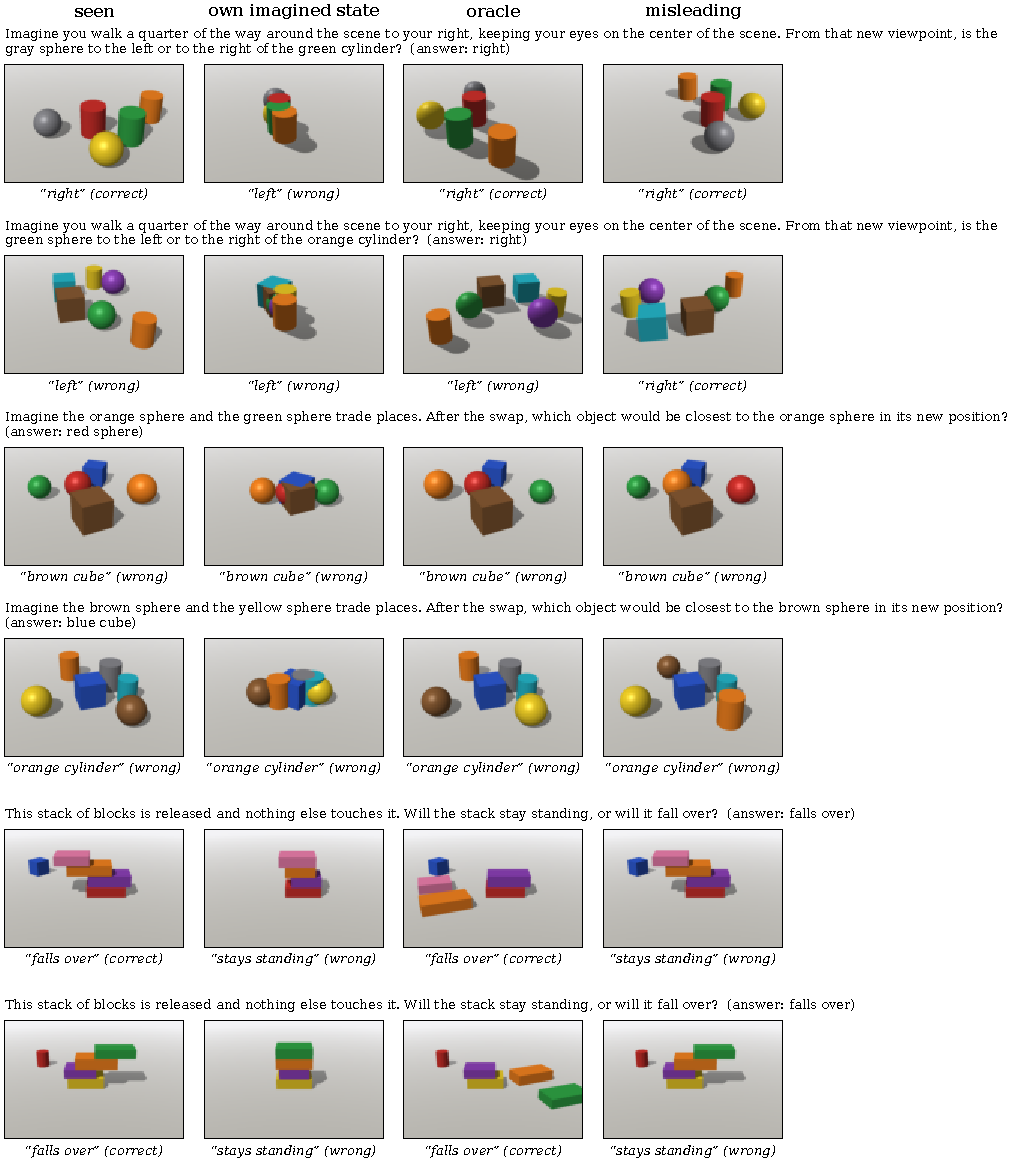
\includegraphics[width=0.86\linewidth]{figs/supp_examples.pdf}
  \captionof{figure}{\textbf{Two questions per task}, with Qwen3-VL-8B's actual answer under each second image (``seen'': the original image only). The examples include failures: on rearrangement the model answers wrongly even with the oracle, and its own reconstructions compress the scene into a cluster (viewpoint) or into a vertical, stable-looking stack (physical outcome).}
  \label{fig:supp-examples}
\end{center}



\end{document}
